
\chapter{Menu Volumes}\label{volumes_chapter}
\minitoc 

\section{Edit first selected volume}
This option opens the "Edit first selected volume" window.
The "Edit first selected" window can also be opened by clicking on "
\includegraphics[scale=0.7]{images/06/objects/volume_edit.png}" (see Fig. \ref{edit_volume_window} p.\pageref{edit_volume_window}).



\begin{figure}
  \centering
  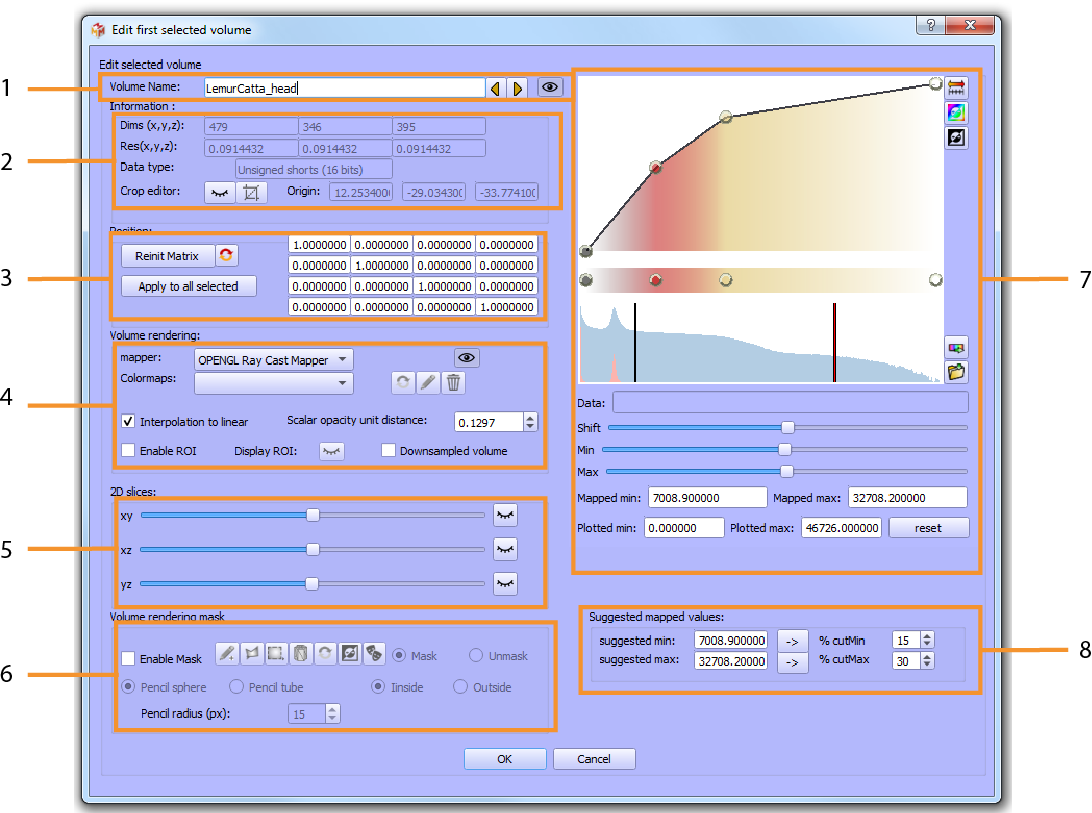
\includegraphics[scale=0.9]{images/14/edit_volume_window.png}
\caption{Edit first selected volume window. This window is divided in different subsections. \textbf{1)} Choose current volume to edit. Change volume name, browse through the different opened volume (arrows), and render or hide the currently activated volume rendering representation and/or 2D slices.  \textbf{2)} Information: dimensions, voxel size and data type of the currently selected volume. Crop editor: define crop region of the currently selected volume. \textbf{3)} Position matrix. Edit manually the position matrix, reinit matrix to identity, refresh matrix, and/or apply edited matrix to all selected volumes. \textbf{4)} Volume rendering. Choose mapper and colormap. Show or hide volume rendering representation. Show only a region of the currently selected volume (Enable ROI and display ROI toggles). \textbf{5)} 2D slices settings and visibility in xy, xz and yz planes. \textbf{6)} Volume rendering masking. Mask must be enabled first to activate the different masking tools : pencil sphere, pencil tube, free-form lasso, square lasso, use 3D surface to mask volume region, invert mask, and fill masked voxels.  \textbf{7)} Color map edition and histogram (orange: linear scale; blue: logarithmic scale). \textbf{8)} Map 3D volume using suggested min and suggested max values.}	
\label{edit_volume_window}
 \end{figure}

\subsection{Volume: name, selection and visibility}
Switching between all currently opened volume, editing their names can be performed in this section (see Fig.\ref{volume_name} p.\pageref{volume_name}).
\begin{figure}
  \centering
  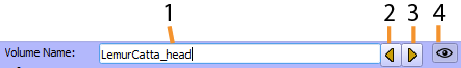
\includegraphics[scale=1]{images/14/volume_name2.png}
\caption{Volume: name, selection and visibility. \textbf{1)} View and/or change the name of the currently selected volume.  \textbf{2)} Select preceding volume.  \textbf{3)} Select next volume. \textbf{4)} make visible or hide all representations in the 3D window for the currently selected volume (volume rendering and/or 2D slices representations). }	
\label{volume_name}
 \end{figure}

In this section you can also decide to show or hid all currently visible representations of the selected volume (volume rendering and xy, yz, xz slices), see Fig.\ref{volume_name_visibility} p.\pageref{volume_name_visiblity}).
\begin{figure}
  \centering
  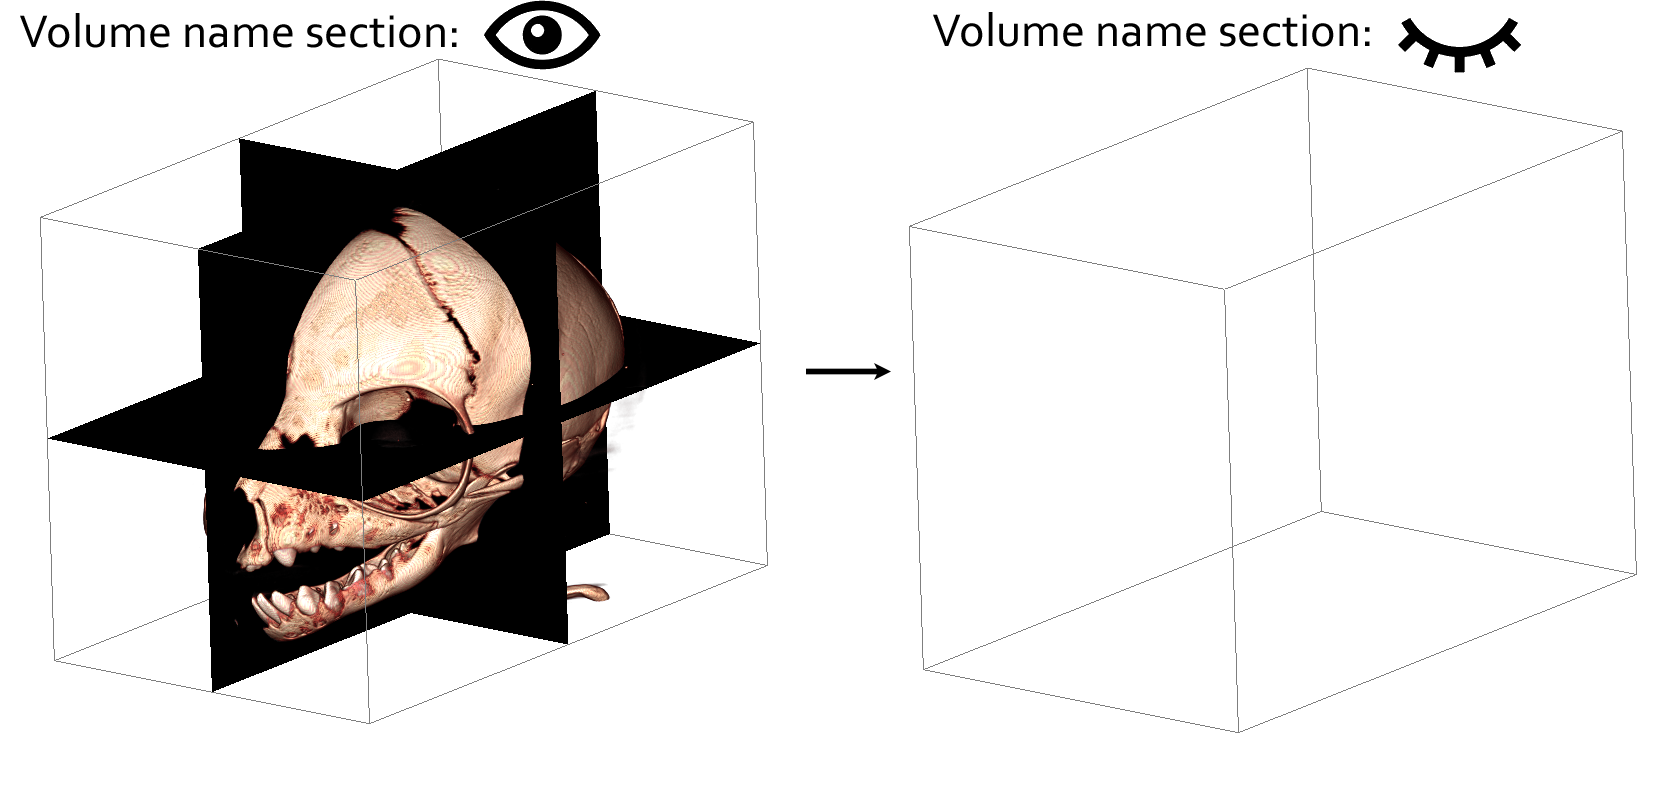
\includegraphics[scale=0.3]{images/14/volume_name/volume_name_visibility.png}
\caption{Visibility. \textbf{Left:} Default behavior: all currently active representations of the selected volume are visible.   \textbf{Right:} all currently active representations of the volume are now hidden.}	
\label{volume_name_visibility}
 \end{figure}


\subsection{Information and crop editor}
Volume dimensions, resolution, data type and position in 3D space of the first voxel of the volume (origin) are available in this section (see Fig. \ref{volume_information} p.\pageref{volume_information}). The crop editor is also situated in this section (see Fig.\ref{crop_example} p.\pageref{crop_example}). 
\begin{figure}
  \centering
  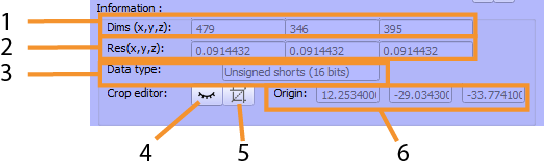
\includegraphics[scale=1]{images/14/volume_information2.png}
\caption{Volume information and crop editor. \textbf{1)} Number of voxels in X, Y and Z dimensions of currently selected volume.   \textbf{2)} Voxel resolution in X, Y and Z (scale: size unit most often expressed in mm). \textbf{3)} Data type (8 bits, 16 bits, 32 bits or 64 bits voxels).  \textbf{4)} Display / hide crop box. \textbf{5)} Apply crop box: restrict the dimensions of the currently opened volume to those of the crop box. \textbf{6)} Origin of the first voxel of currently selected volume in X,Y and Z. }	
\label{volume_information}
 \end{figure}


\begin{figure}
  \centering
  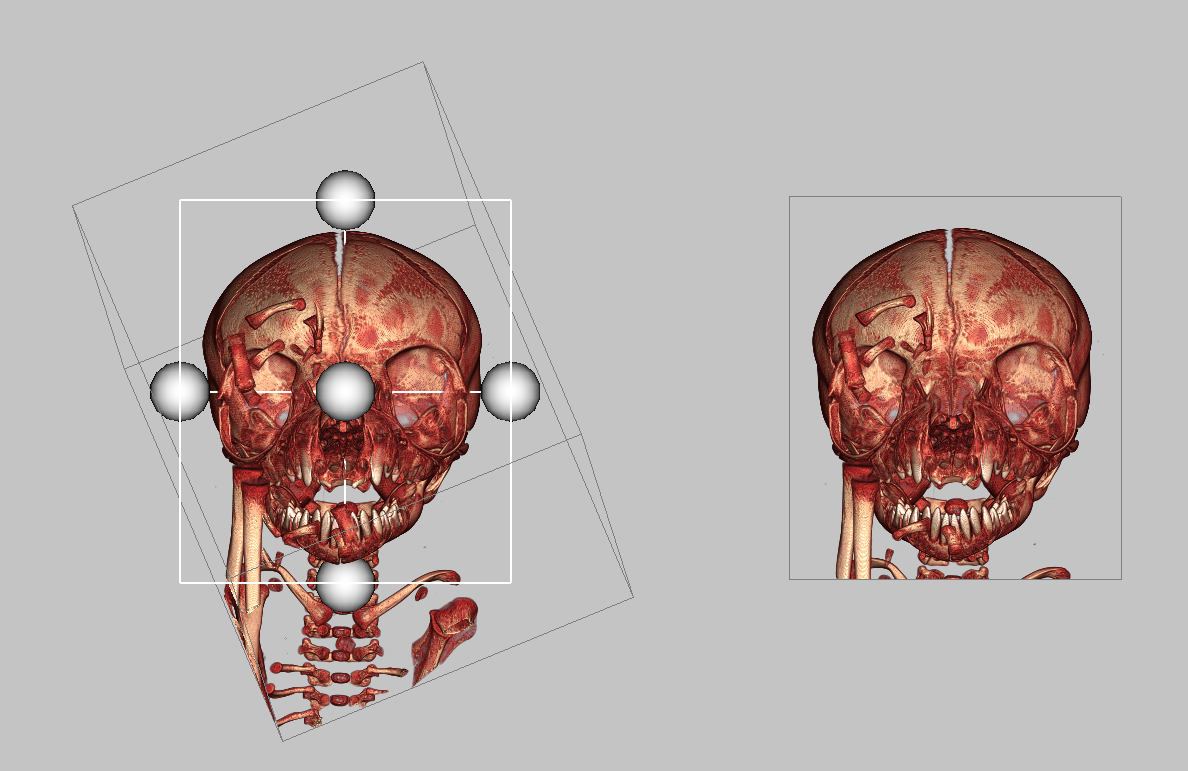
\includegraphics[scale=0.4]{images/14/crop_example/crop_example.png}
\caption{Cropping volumes. \textbf{Left:} Crop box definition of a rotated volume. When volumes have been rotated, "cropping" will performed after reslicing the volume.   \textbf{Right:} Resliced + cropped result.}	
\label{crop_example}
 \end{figure}

\subsection{Position}
Volume position matrix can be manually edited, reinitialized and refreshed inside this section (see Fig. \ref{volume_position} p. \pageref{volume_position}).
\begin{figure}
  \centering
  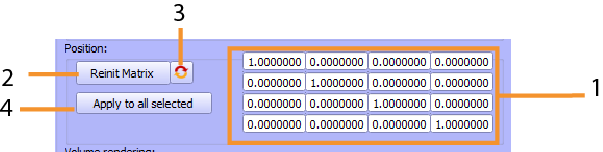
\includegraphics[scale=1]{images/14/volume_position2.png}
\caption{Volume position section. \textbf{1)} Position matrix.   \textbf{2)} Reset position matrix to identity. \textbf{3)} Refresh position matrix.  \textbf{4)} Apply position matrix to all selected volumes. }	
\label{volume_position}
 \end{figure}



\subsection{Volume rendering}
Volume rendering options are located in this section (see Fig. \ref{volume_rendering} p. \pageref{volume_rendering}).
\begin{figure}
  \centering
  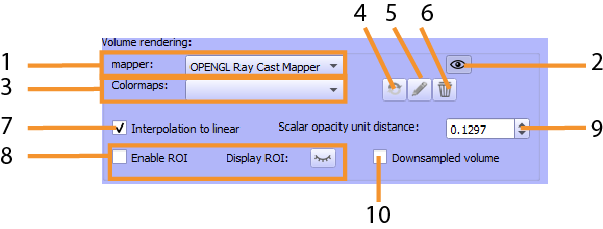
\includegraphics[scale=1]{images/14/volume_rendering2.png}
\caption{Volume rendering section. \textbf{1)} Chose mapper (note that "Smart Volume mapper" does not currently allow masks).   \textbf{2)} Display / hide volume rendering representation of currently selected volume. \textbf{3)} Change color map.  \textbf{4)} Reinitialize current colormap (only possible for default colormaps). \textbf{5)} edit current colormap name (only possible for user-defined colormaps.) \textbf{6)}delete current colormap (only possible for user-defined colormaps.) \textbf{7)} Activate/ deactivate linear interpolation rendering. \textbf{8)} Enable/ disable ROI clipping box, and display / hide clipping box boundaries and edition handles.  \textbf{9)} Change scalar opacity unit distance. \textbf{10)} Render a down-sampled version of the currently selected volume rather than the full volume (large volumes, e.g. > 1Gb datasets are often hard to render on standard graphics cards and may make your computer crash).  }	
\label{volume_rendering}
 \end{figure}

Different colormaps are available inside the Colormaps combobox, and you may also add custom colormaps. How changing colormaps affects volume rendering representations is illustrated Fig. \ref{volume_colormap_example} p. \pageref{volume_colormap_example}.
\begin{figure}
  \centering
  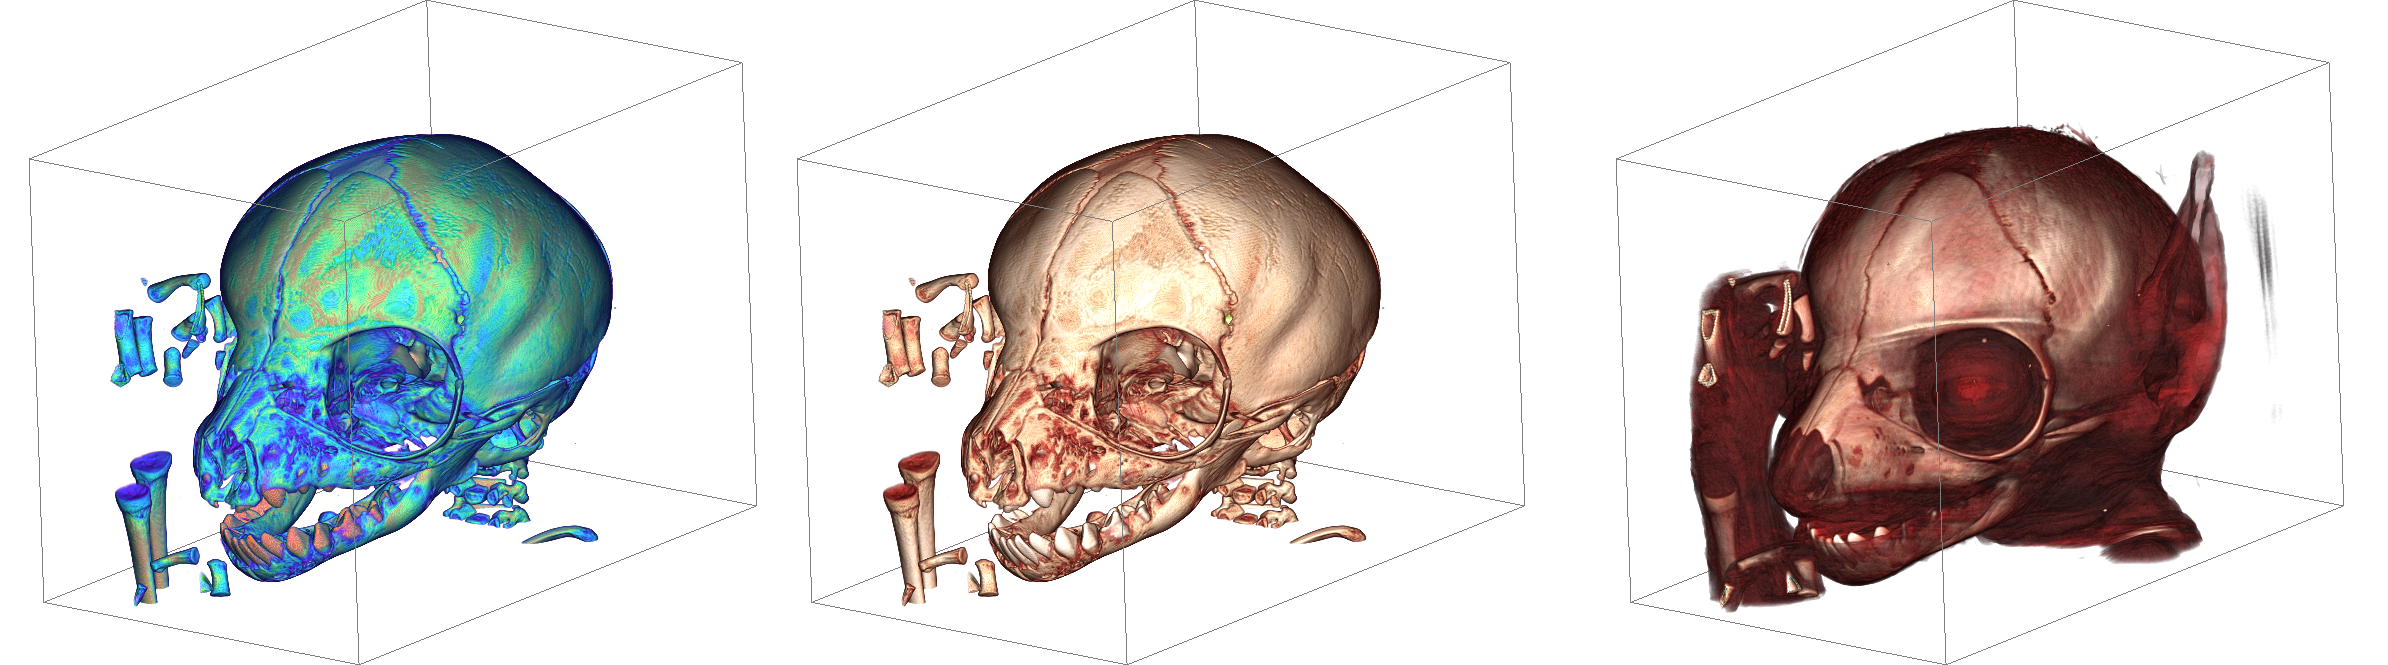
\includegraphics[scale=0.2]{images/14/colormap_example/colormap_example.png}
\caption{Colormaps. \textbf{Left:} Volume rendering using the rainbow colormap. \textbf{Center:} Volume rendering using the Black-red-white colormap.  \textbf{Right:}Volume rendering using also the Black-red-white colormap, after the mapped min and mapped max values have been shifted.}	
\label{volume_colormap_example}
 \end{figure}

The scalar opacity unid distance (SOUD) parameter also dramatically affects volume rendering representations. For a given volume, MorphoDig initializes this parameter as a fraction of the length of diagonal of the bounding box of that volume. However, you may decide to adjust this parameter manually (see for instance Fig. \ref{soud_example} p. \pageref{soud_example}).
\begin{figure}
  \centering
  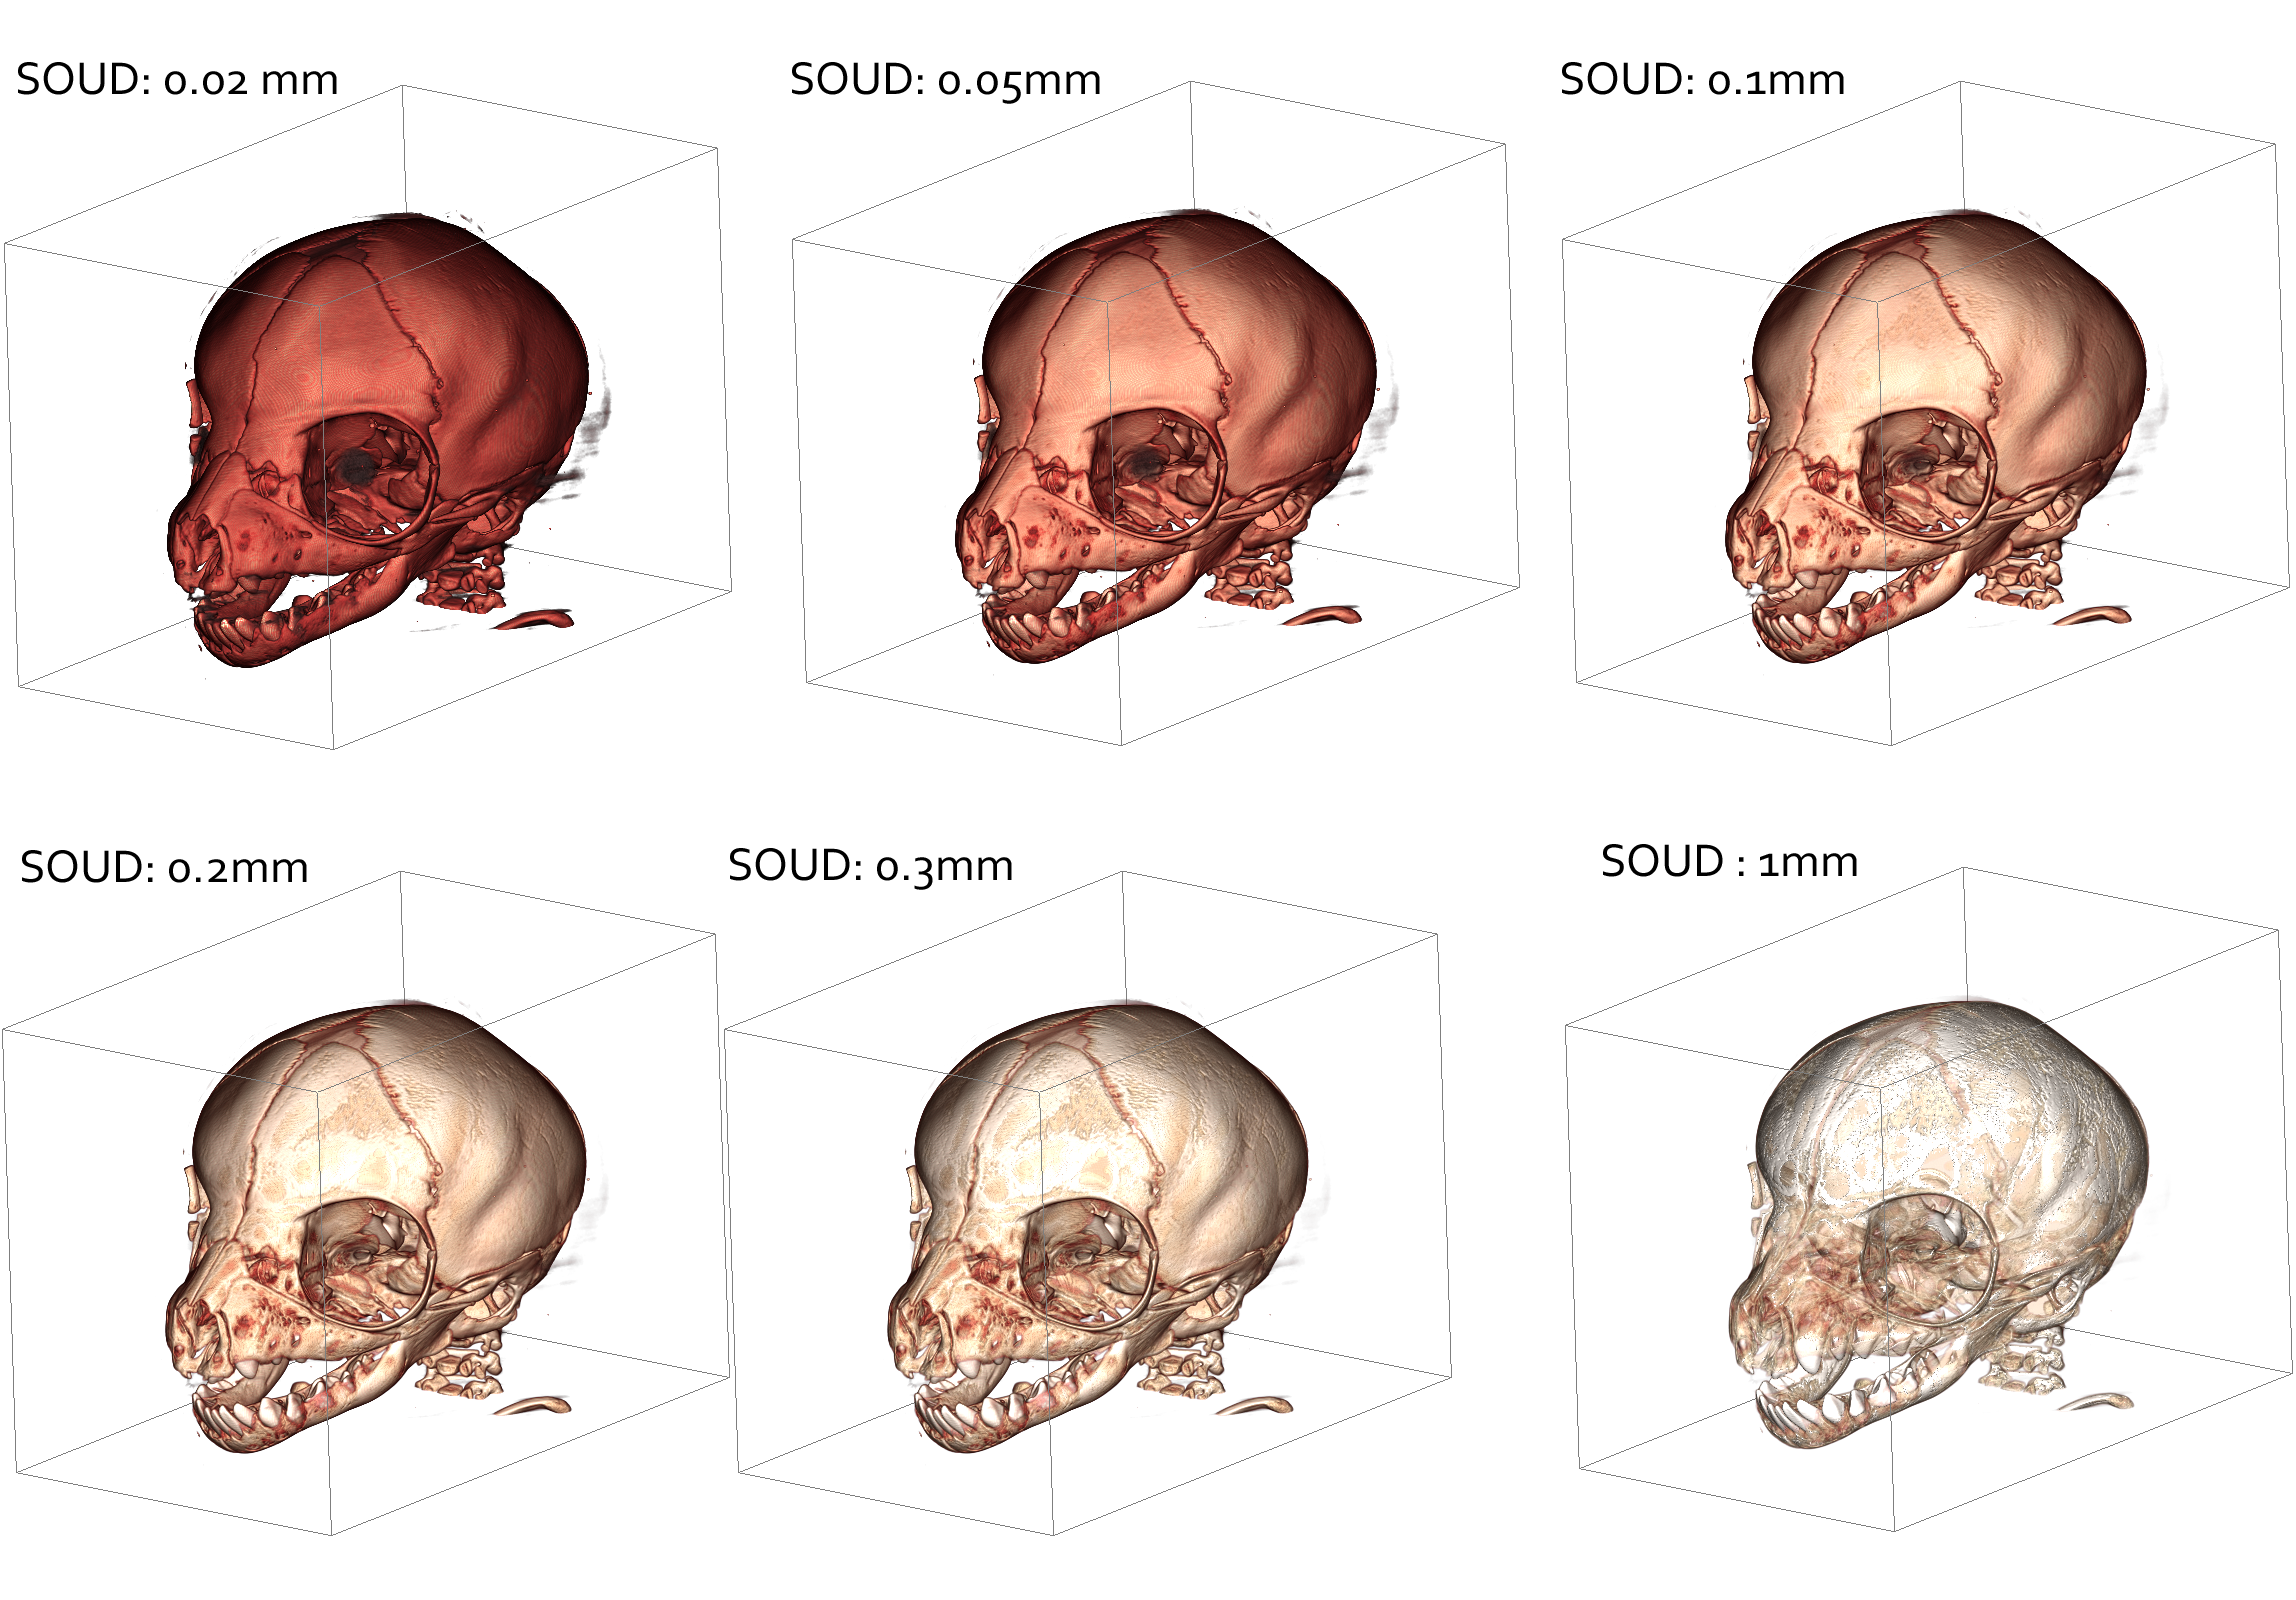
\includegraphics[scale=0.21]{images/14/soud/soud_example.png}
\caption{Scalar Opacity Unit Distance (SOUD) dramatically affects volume rendering representations. For a given volume, MorphoDig initializes this parameter as a fraction of the length of diagonal of the bounding box. However, as illustrated here, you may decide to adjust SOUD manually.}	 
\label{soud_example}
 \end{figure}


\subsection{2D slices}
Display of 2D slices inside the 3D main window is located in this section (see Fig. \ref{volume_2Dslices} p. \pageref{volume_2Dslices}).
\begin{figure}
  \centering
  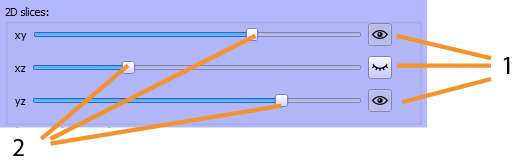
\includegraphics[scale=1]{images/14/volume_2Dslices2.png}
\caption{2D slices  \textbf{1)} Display / hide 2D slices in xy, xz and yz planes. \textbf{2)} Change slice number in xy, xz and yz planes.  }	
\label{volume_2Dslices}
 \end{figure}
By default, the volume rendering representation is activated, and hides very much the 2D slices. In order to improve the visibility of the 2D slices representations, the volume rendering representation may be hidden (see Fig. \ref{2D_slices_example} p. \pageref{2D_slices_example}).
\begin{figure}
  \centering
  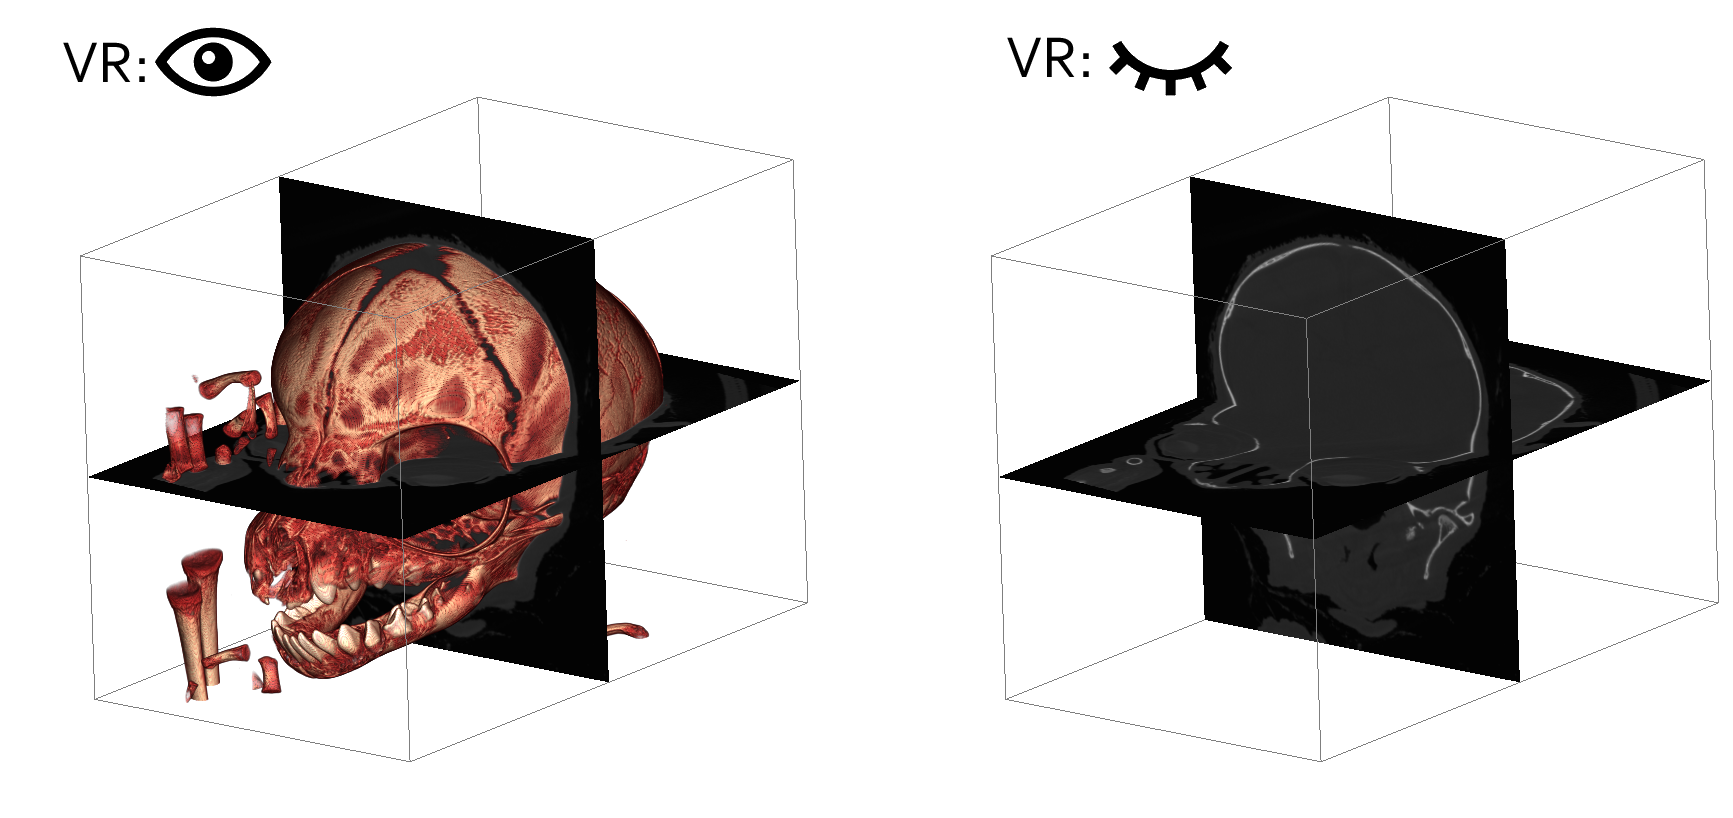
\includegraphics[scale=0.3]{images/14/2Dslices_example/2Dslices_example.png}
\caption{2D slices representation. \textbf{Left:} by default, the volume rendering representation is activated, and hides very much the 2D slices. \textbf{Left:} hiding the volume rendering representation improves the visibilty of the 2D slices.}	 
\label{2D_slices_example}
 \end{figure}

\subsection{Volume rendering mask}\label{volume_rendering_masking}
Volume rendering masking tools are located in this section (see Fig. \ref{volume_masking} p. \pageref{volume_masking}). Note that when the Smart Volume Mapper is selected, masking tools become unavailable.
\begin{figure}
  \centering
  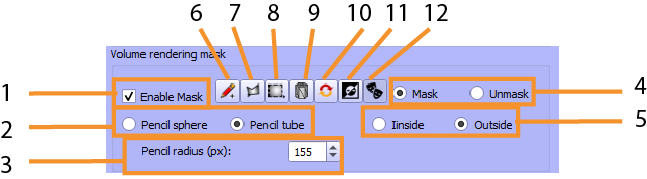
\includegraphics[scale=1]{images/14/volume_masking2.png}
\caption{Volume rendering mask.  \textbf{1)} Enable/disable mask tools. \textbf{2)} When using the pencil tool, choose between spherical shape and cylindric shape.  \textbf{3)} Define pencil radius in terms of screen pixels. Pencil radius can be interactively changed by keeping "T" pressed while rolling the middle mouse button.  \textbf{4)} Define whether voxels laying inside the selection should be masked or unmasked. \textbf{5)} Define whether selected voxels to mask/unmask laying inside or outside the selected region. \textbf{6)} Pencil selection tool. \textbf{7)} Lasso selection tool. \textbf{8)} Rectangular region selection tool.  \textbf{9)} 3D surface selection tool: use a 3D surface to define which region should be masked. \textbf{10)} Reinitialize mask. \textbf{11)} Invert mask. \textbf{12)} Harden transform mask. \textbf{13)} Import mask. \textbf{14)} Export mask.}	
\label{volume_masking}

 \end{figure}
Different examples are provided:\\
Masking using the \textbf{pencil} tool is presented Fig. \ref{mask_pencil} p.\pageref{mask_pencil}\\
Masking using the \textbf{lasso} is presented Fig.\ref{mask_lasso} p.\pageref{mask_lasso}\\
Masking using the \textbf{rubber band} (rectangular selection) is presented Fig.\ref{mask_rubber} p. \pageref{mask_rubber}\\
Masking using a \textbf{3D surface} (in this example: a spherical surface) is presented Fig.\ref{mask_sphere} p. \pageref{mask_sphere}\\
Mask \textbf{inversion} is presented Fig.\ref{invert_mask} p. \pageref{invert_mask}\\
Mask \textbf{hardening} is presented Fig.\ref{harden_example} p. \pageref{harden_example}\\

\begin{figure}
  \centering
  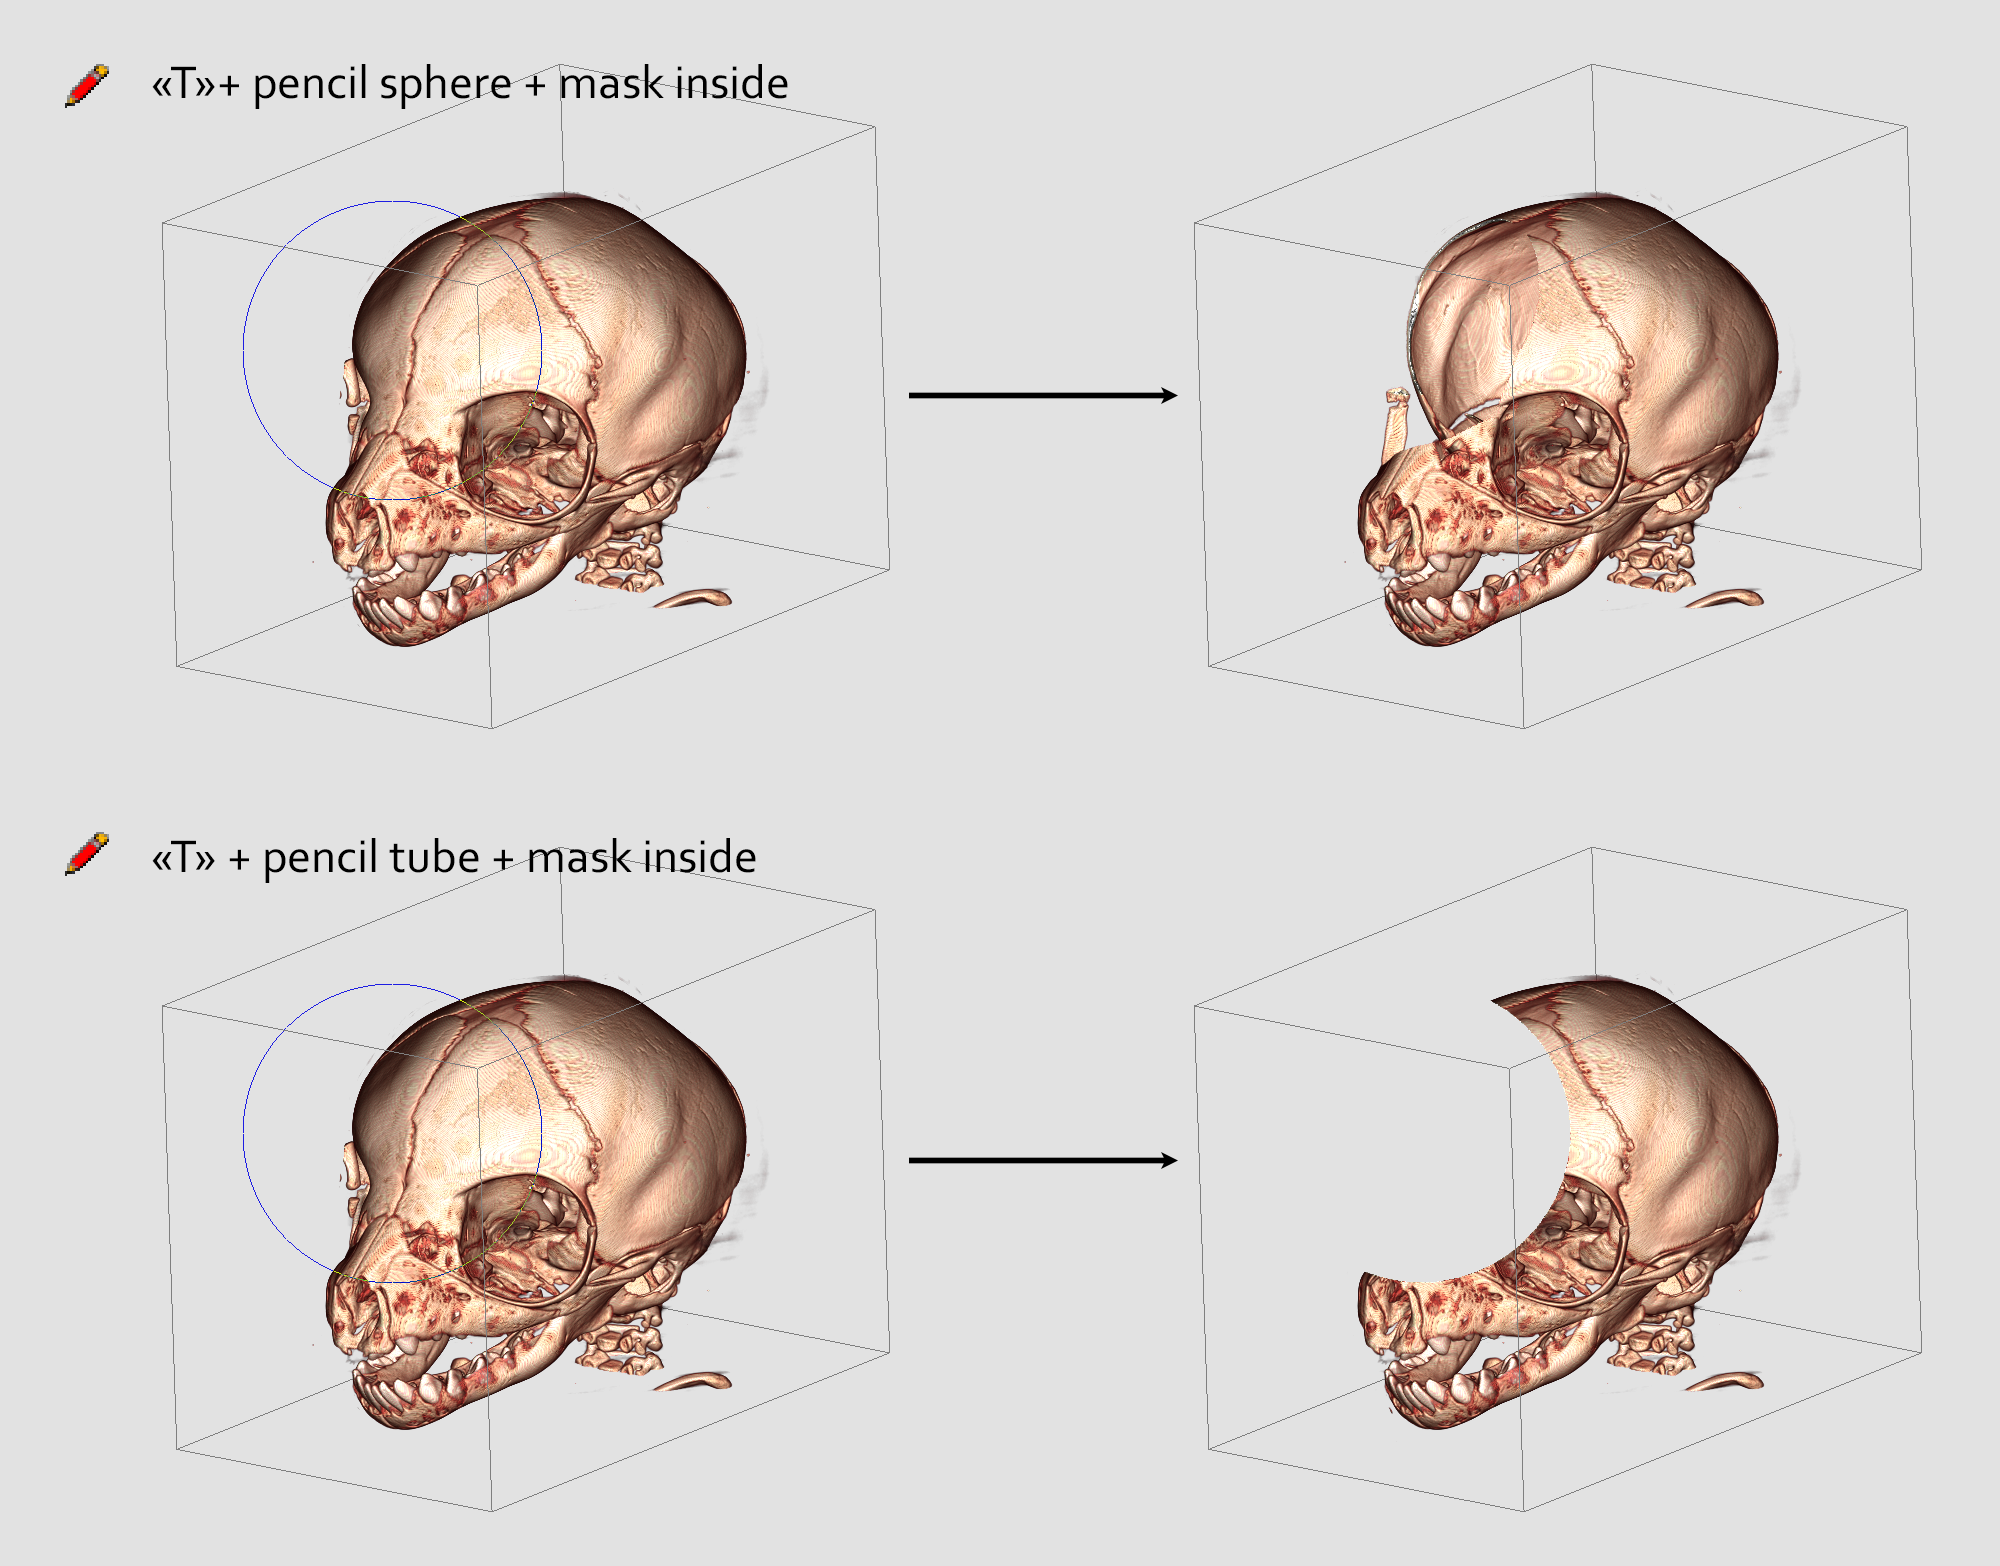
\includegraphics[scale=0.25]{images/14/mask_example/mask_pencil.png}
\caption{Masking using the pencil tool. To activate the pencil, keep "T"  pressed and use the mouse left click. \textbf{Top line:} when the pencil sphere option is  chosen, the masked region has a spherical shape. \textbf{Bottom:} When the pencil tube option is chosen, the masked region has a cylindrical shape.}	 
\label{mask_pencil}
 \end{figure}

\begin{figure}
  \centering
  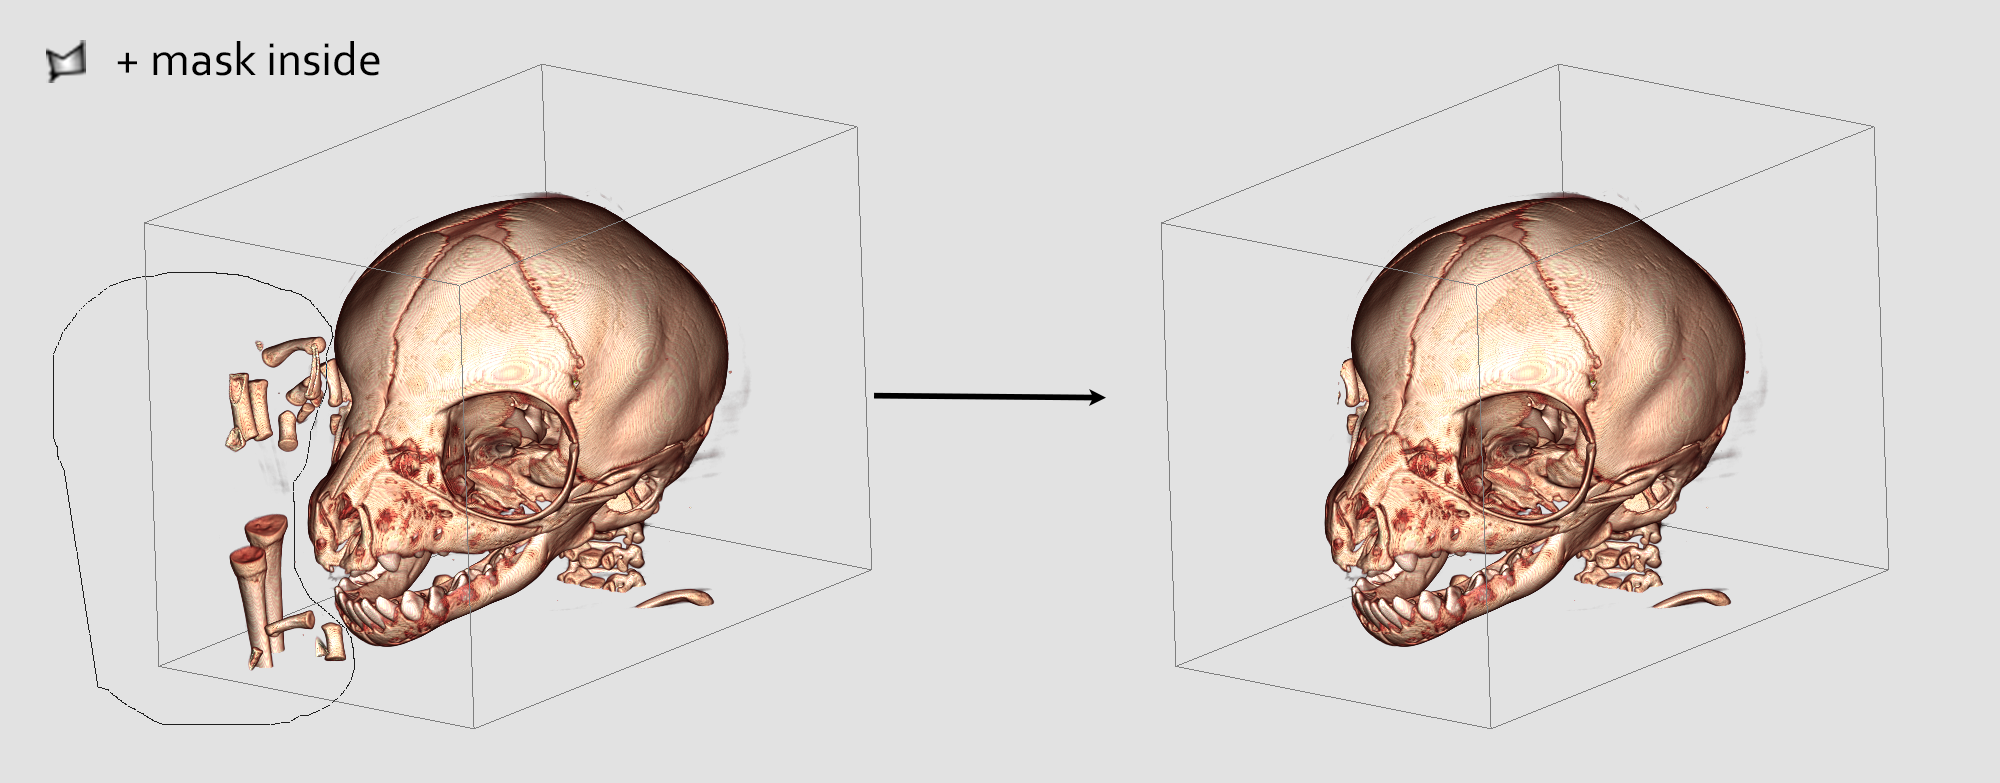
\includegraphics[scale=0.25]{images/14/mask_example/mask_lasso.png}
\caption{Masking using the lasso tool.  \textbf{Left:} First draw a zone to mask (mouse left click maintained + drag). When done, release left mouse button \textbf{Right:} Result (mask inside option was chosen).}	 
\label{mask_lasso}
 \end{figure}

\begin{figure}
  \centering
  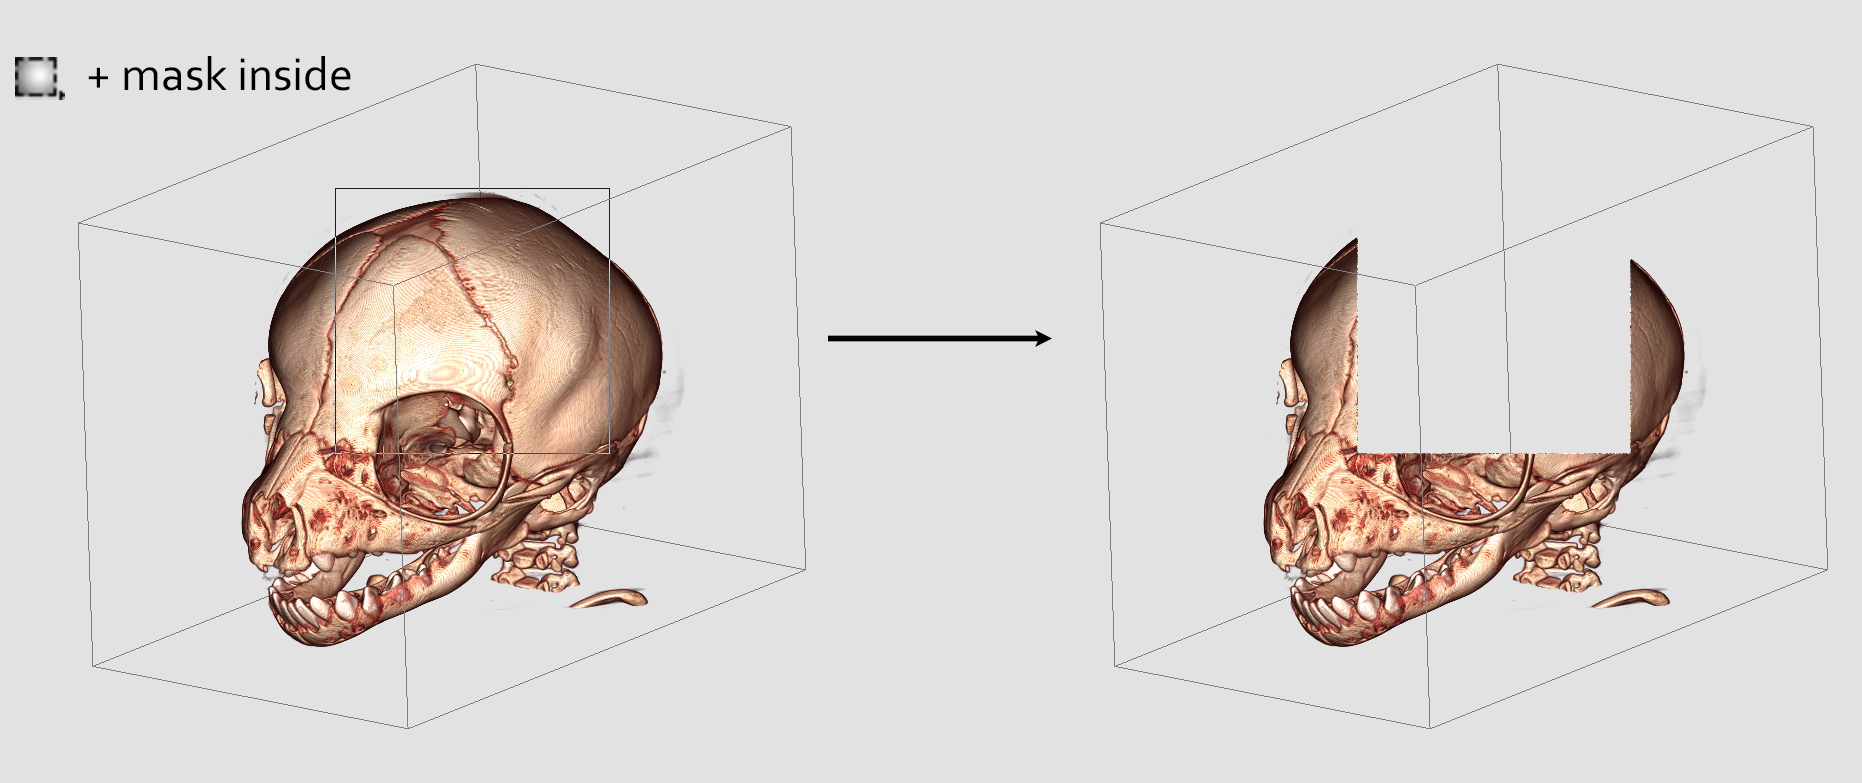
\includegraphics[scale=0.25]{images/14/mask_example/mask_rubber.png}
\caption{Masking using the rubber tool.  \textbf{Left:} First draw a zone to mask (mouse left click maintained + drag). When done, release left mouse button \textbf{Right:} Result (mask inside option was chosen).}	 
\label{mask_rubber}
 \end{figure}


\begin{figure}
  \centering
  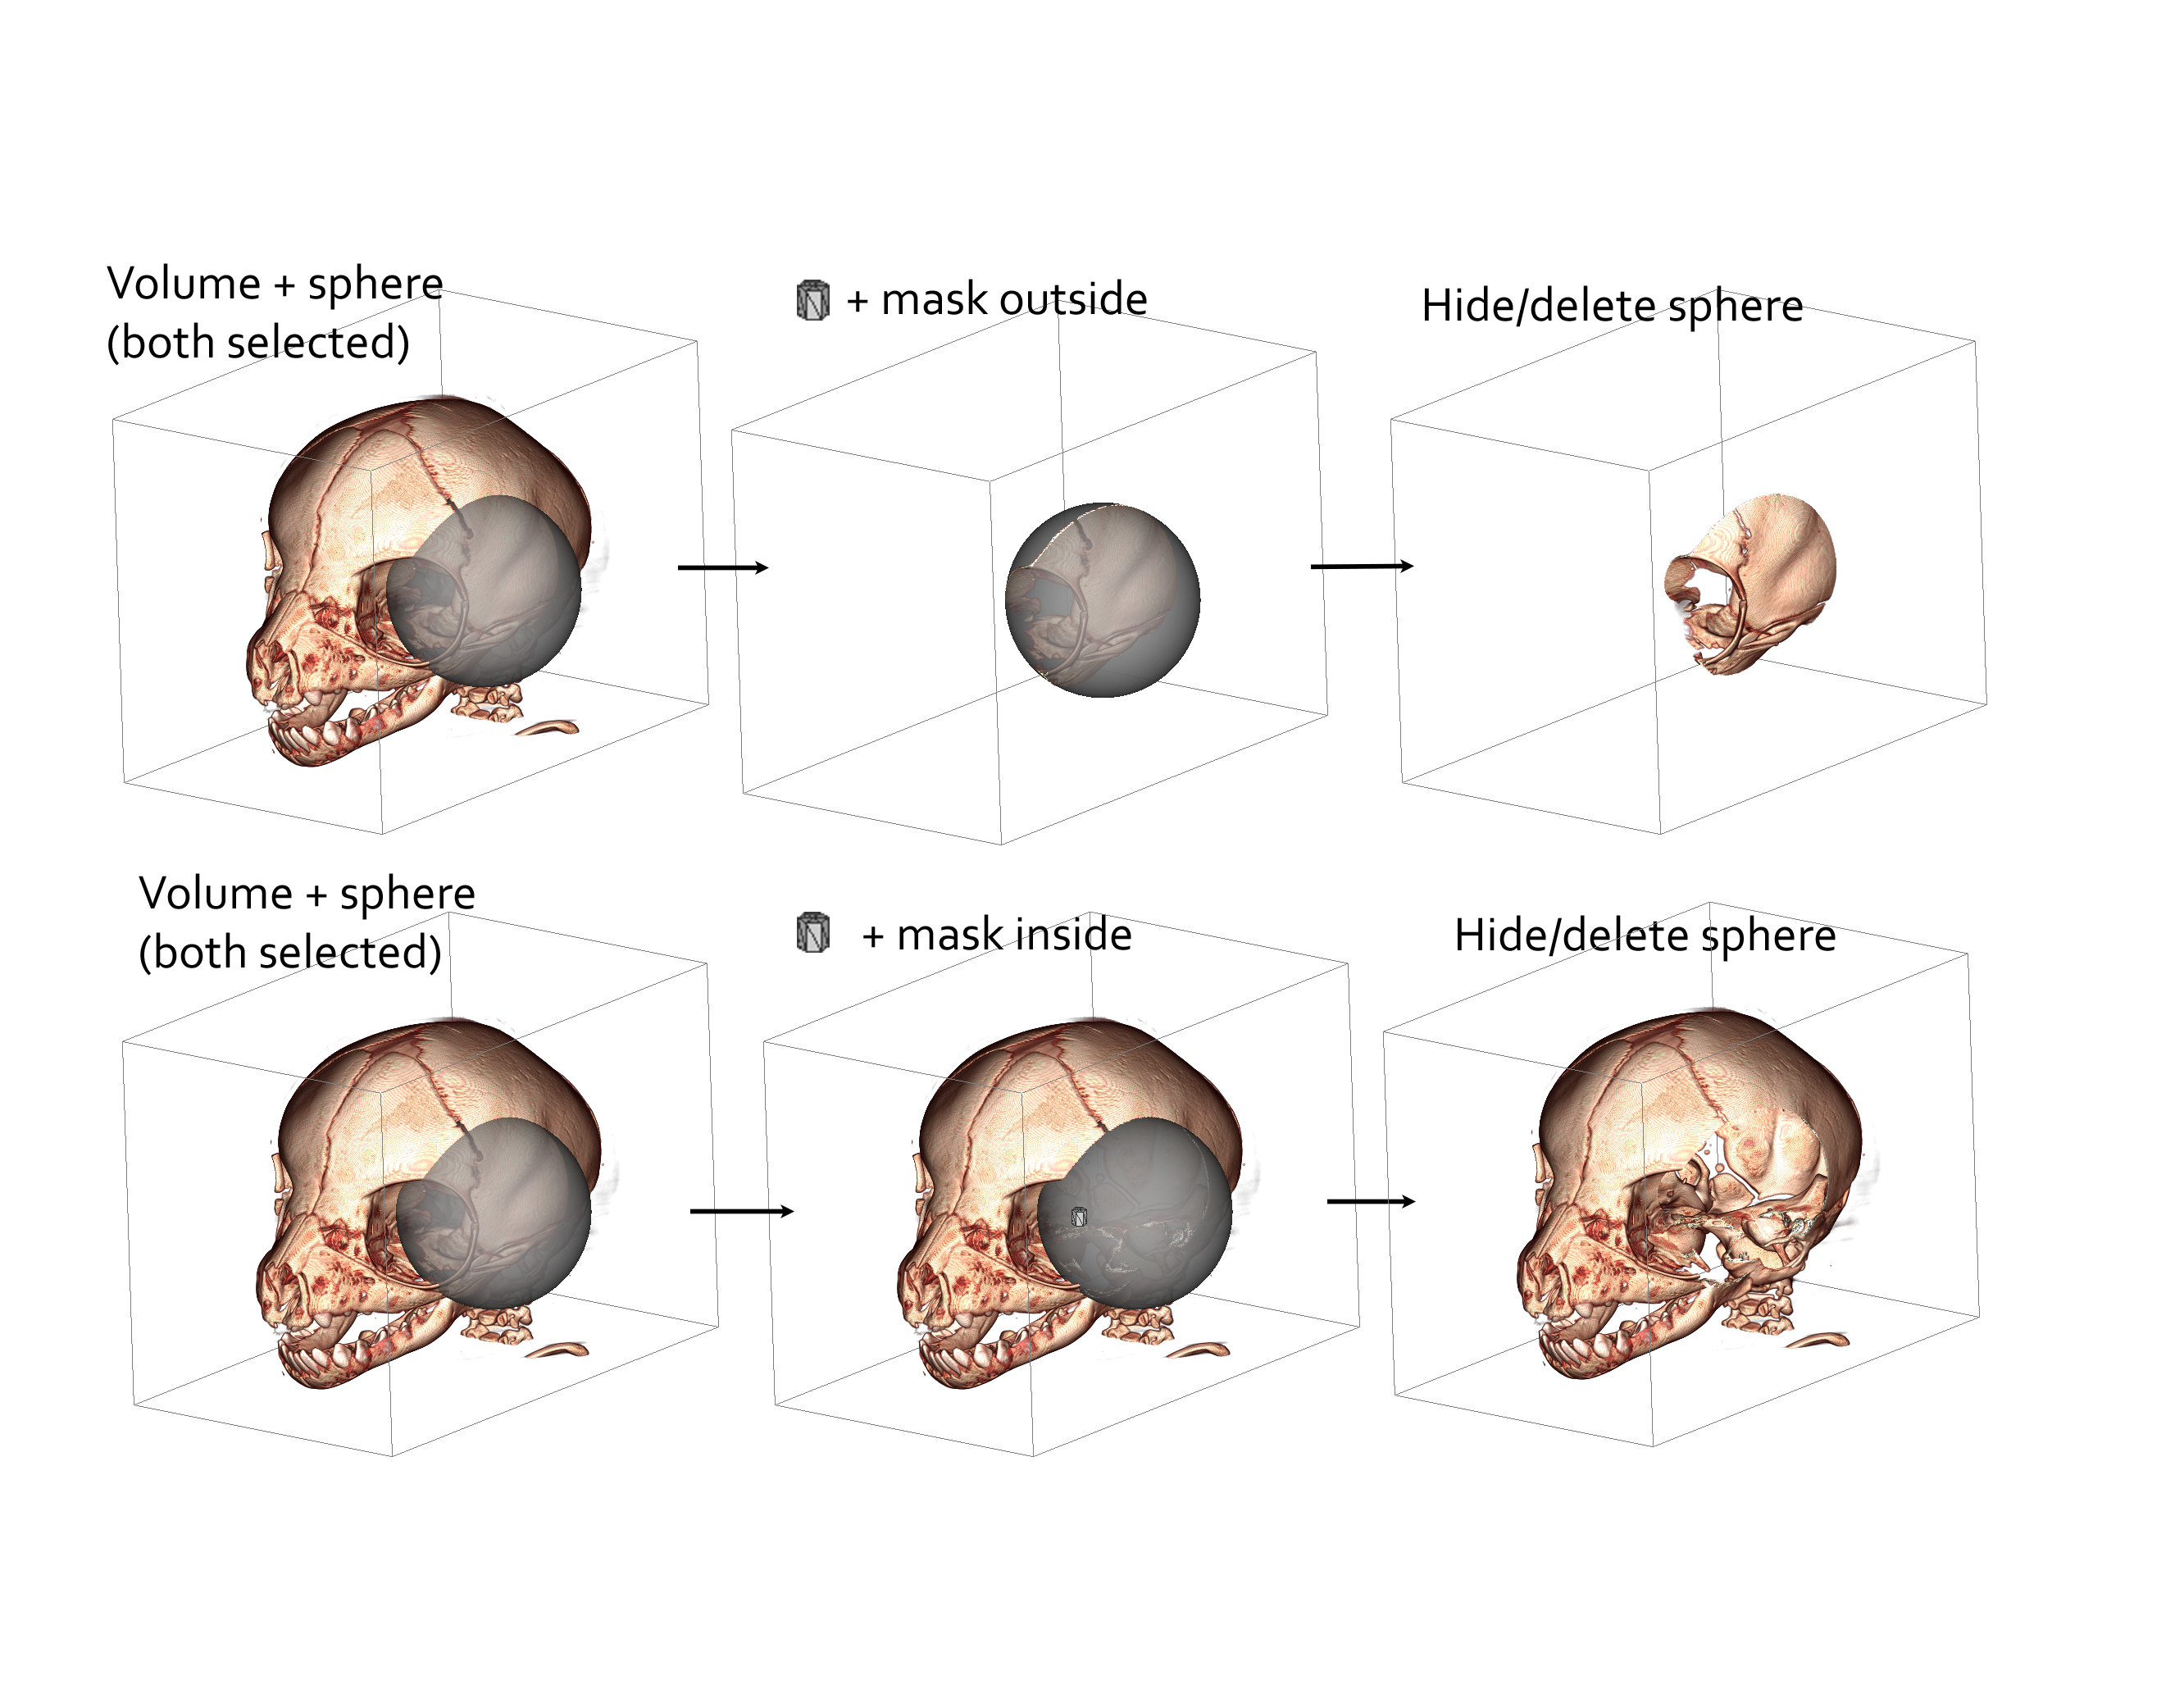
\includegraphics[scale=0.2]{images/14/mask_example/mask_sphere.png}
\caption{Masking using a spherical surface.  \textbf{Top line:} mask inside the region defined by the outise of the sphere. \textbf{Bottom line:} mask inside the region defined by the inside of the sphere.}	 
\label{mask_sphere}
 \end{figure}


\begin{figure}
  \centering
  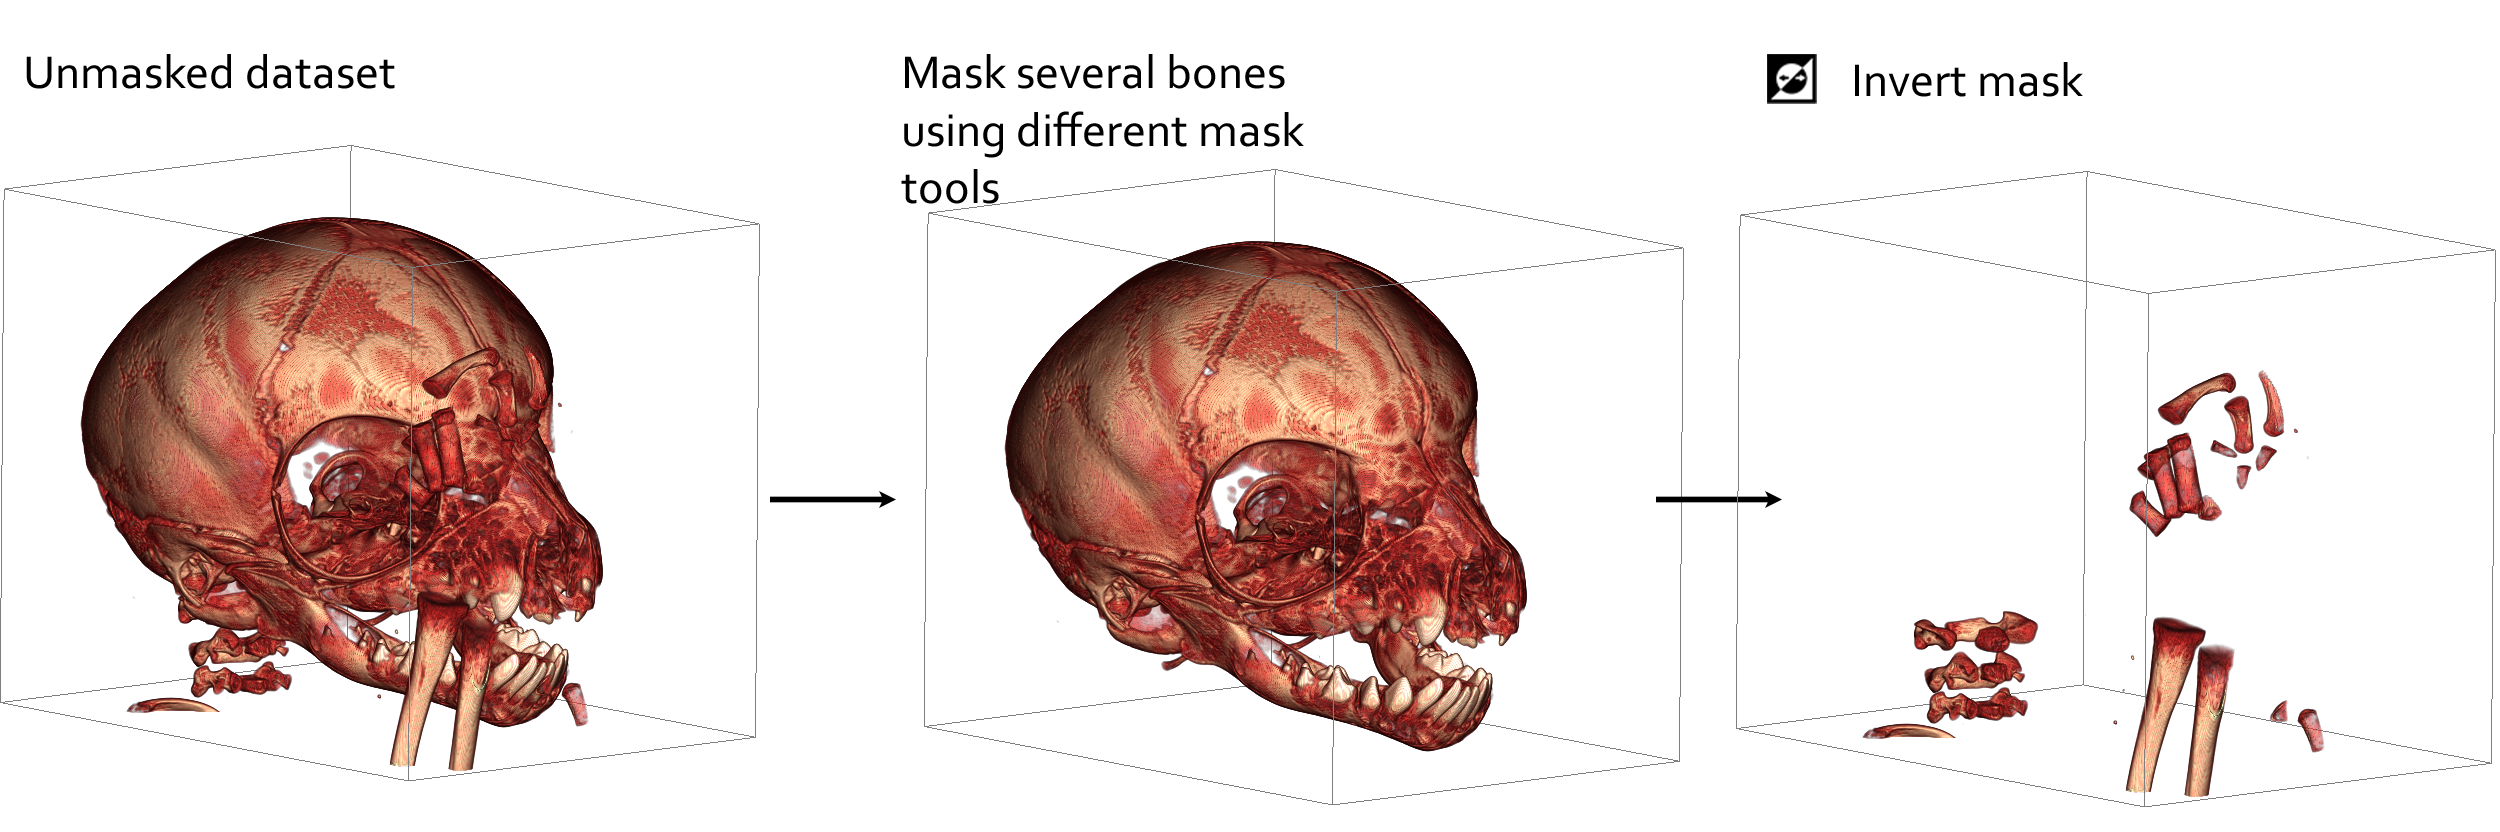
\includegraphics[scale=0.2]{images/14/invert_mask/invert_mask.png}
\caption{Mask inversion.  \textbf{Left} Volume rendering of the full dataset. \textbf{Middle} Several regions were masked using different masking tools. \textbf{Right} All regions that were hidden are visible, and all regions that were visible are now masked.}	 
\label{invert_mask}
 \end{figure}

\begin{figure}
  \centering
  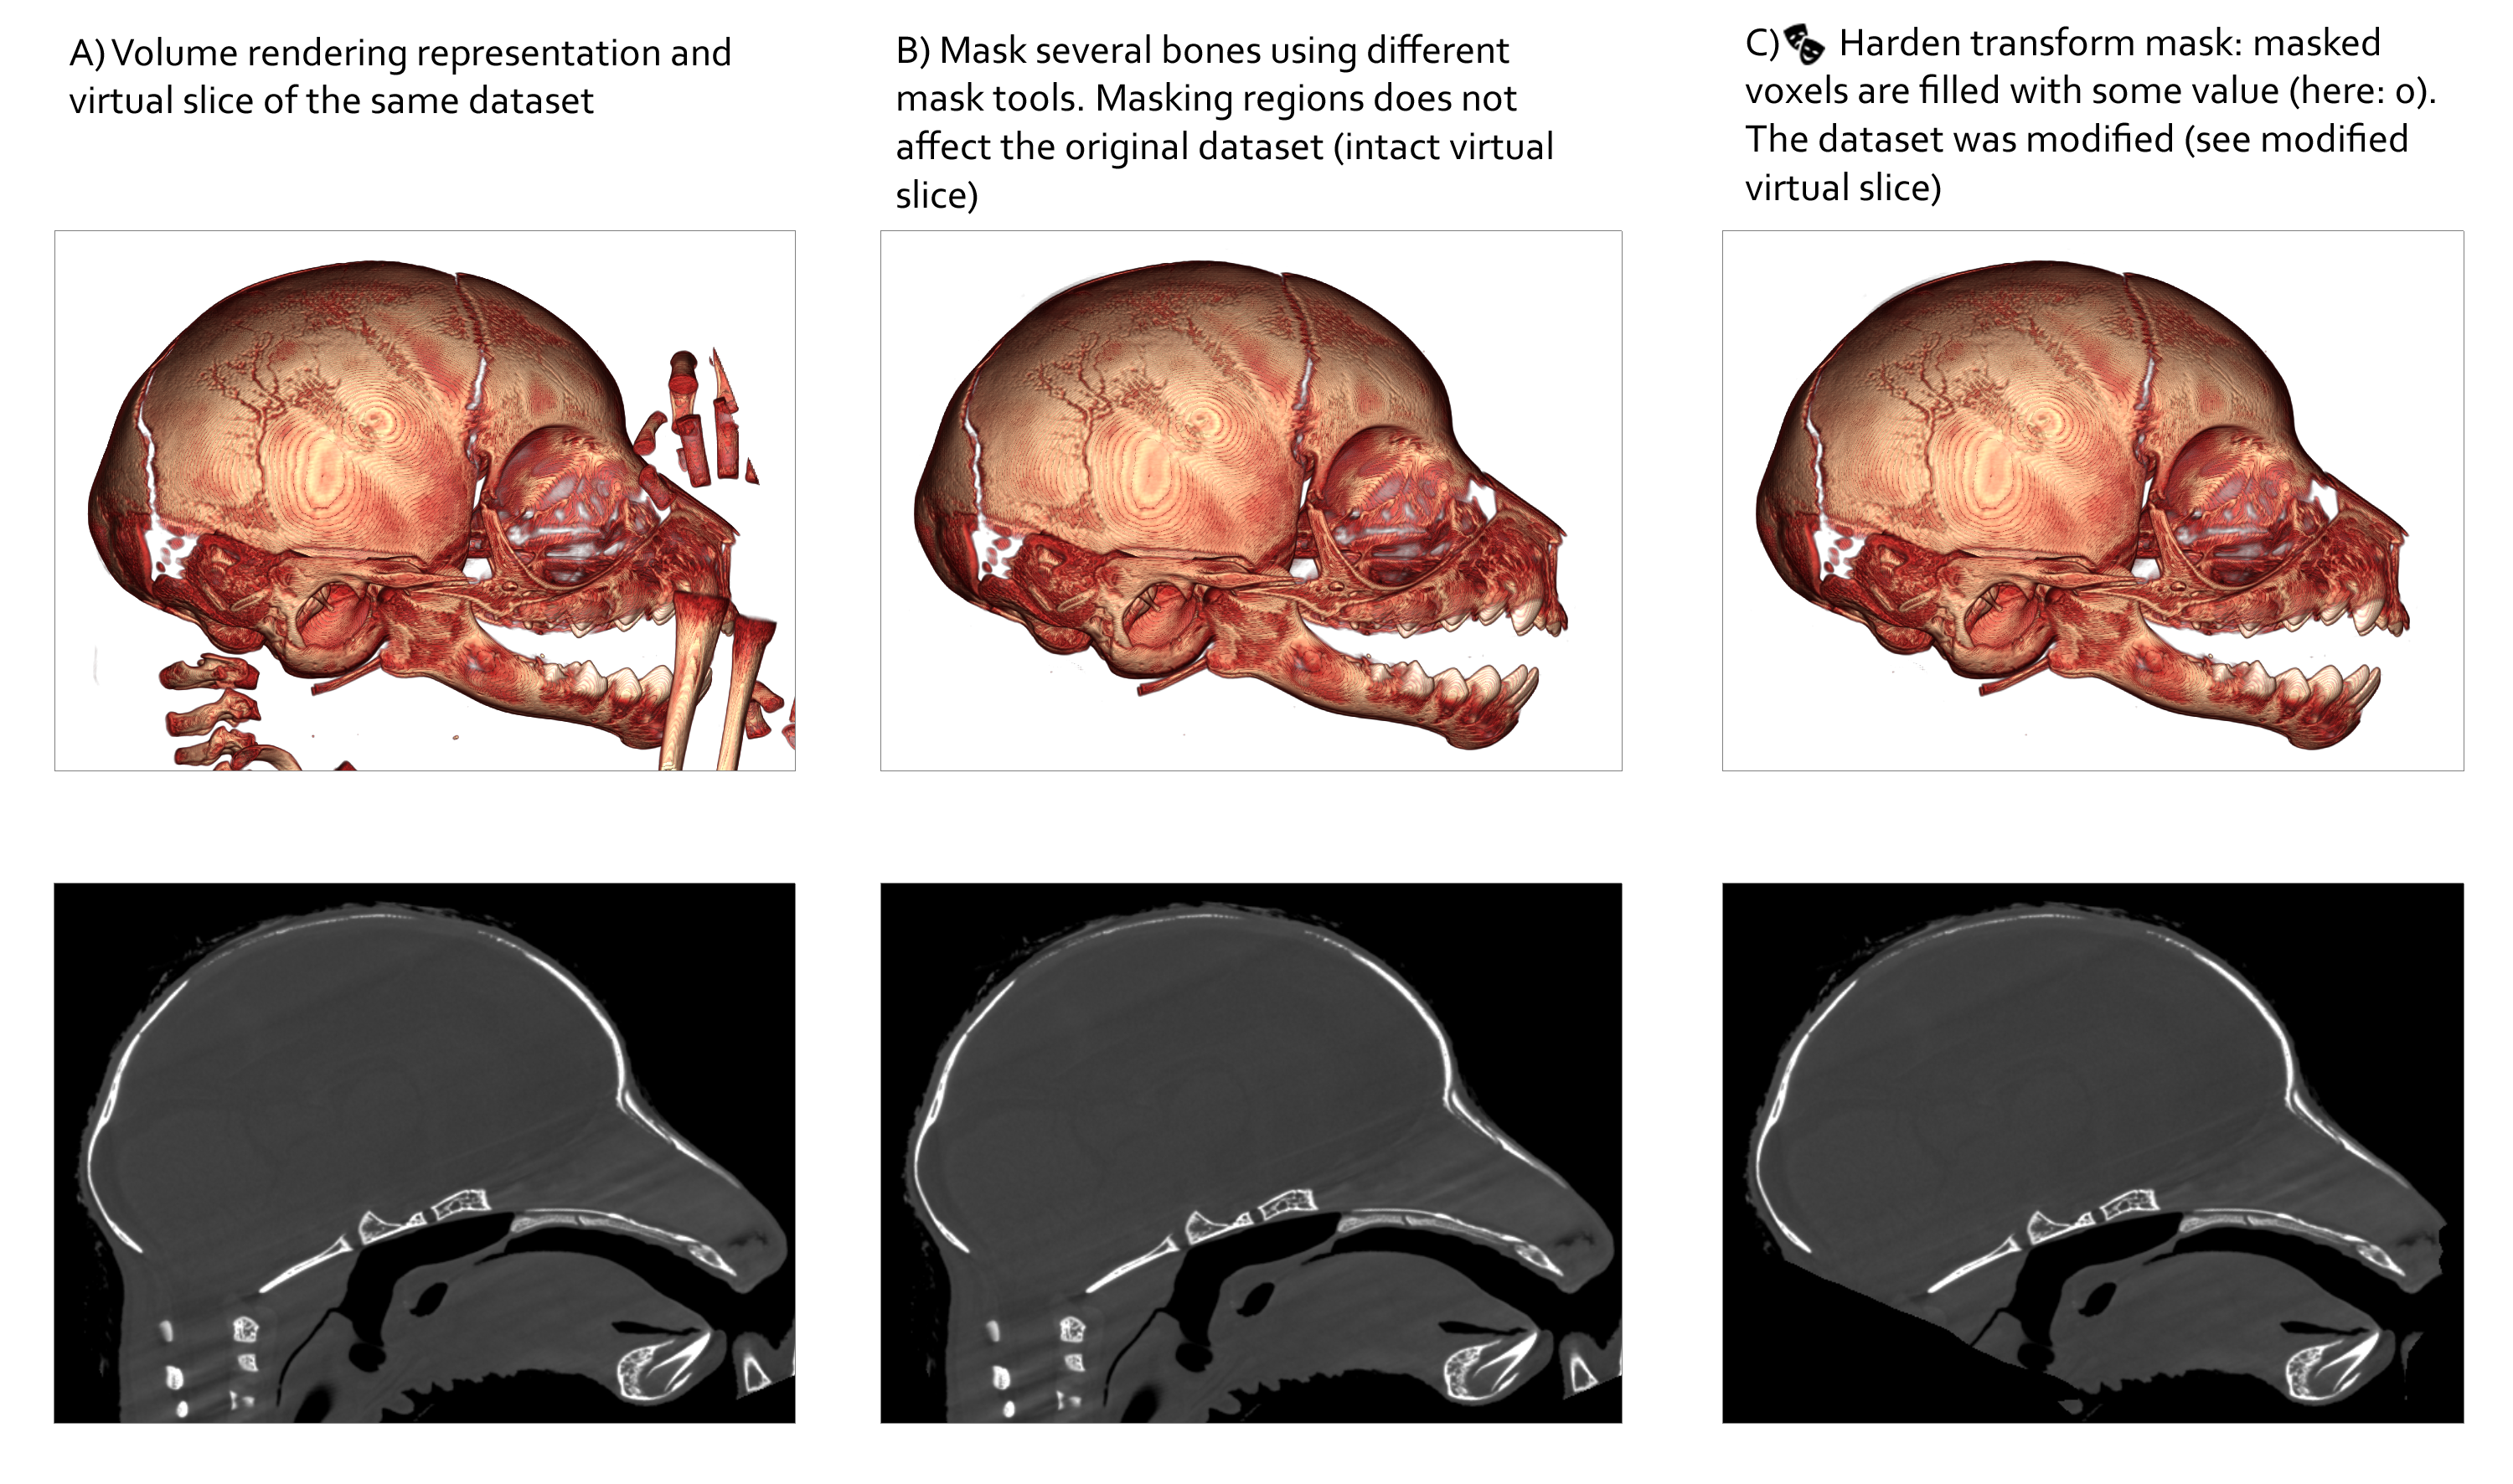
\includegraphics[scale=0.17]{images/14/harden_mask/harden_example.png}
\caption{Mask harden transform.  \textbf{A)} Volume rendering of the full dataset, and Virtual slice. \textbf{B)} Several regions were masked using different masking tools. Note that the virtual slice remains unchanged, which indicates that the original dataset remains intact. \textbf{C)} All previously masked voxels are now given the same value (in that case: "0"): the original data is now modified.}	 
\label{harden_mask}
 \end{figure}



\subsection{Color map edition}
Volume rendering color map edition controls tools are located in this section (see Fig. \ref{volume_colormap} p. \pageref{volume_colormap}). 
\begin{figure}
  \centering
  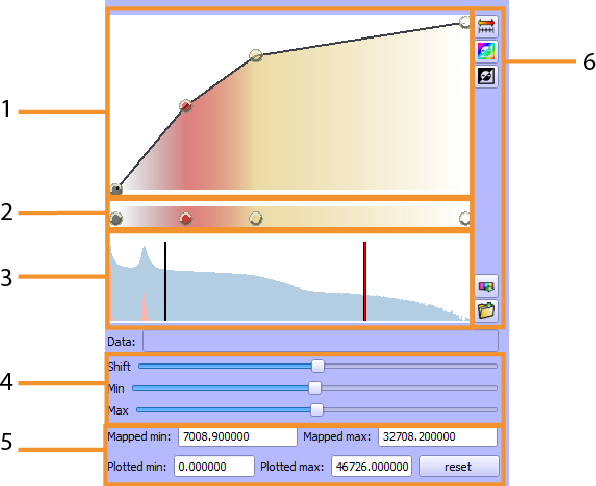
\includegraphics[scale=1]{images/14/volume_colormap2.png}
\caption{Volume rendering colormap control section. \textbf{1)} Opacity control points of the active color map (move these points to change opacity). \textbf{2)} Color control points of the active color map (double click on each point to edit the color). \textbf{3)} Histogram of currently selected volume. Orange: conventional histogram. Blue: logarithmic-scaled histogram. The 2 vertical bars indicate the min and max display range of the colormap.  \textbf{4)} Shift color map display range, or change min and max display range.\textbf{5)} Edit manually mapped min or max value. Edit manually histogram plotted min or max. \textbf{6)} From top to down. a: set range to min and max. b: reverse color control points. c: reverse opacity control points. d: Export colormap to file. e: Save colormap to presets = duplicate current active color map and create a new custom color map.}	
\label{volume_colormap}
 \end{figure}

 How shifting min and max display range affects volume rendering representations is illustrated Fig. \ref{volume_colormap_example} p. \pageref{volume_colormap_example}.

\subsection{Suggested mapped values}
You may decide to reset min and max of the color map based on suggested values. These suggested min and max values are computed in order to remove a percentage of most extreme minimal and maximal values found in the voxels of the currently opened volume (see Fig. \ref{volume_suggested_values} p. \pageref{volume_suggested_values}).
\begin{figure}
  \centering
  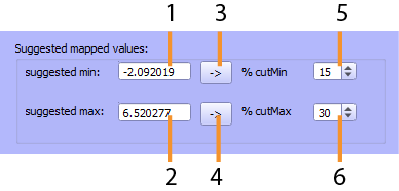
\includegraphics[scale=1]{images/14/volume_suggested_values2.png}
\caption{Volume rendering suggested mapped values. \textbf{1)} Suggested minimal value. \textbf{2)} Suggested maximal value. \textbf{3)} Apply suggested min value.  \textbf{4)} Apply suggested max value.\textbf{5)} Change the percentage of extreme minimal values to compute a new suggested minimal value. \textbf{6)} Change the percentage of extreme maximal values to compute a new suggested maximal value.}	
\label{volume_suggested_values}
 \end{figure}


\section{Extract isosurface from first selected volume}
This option opens the "Isosurface" dialog (see Fig. \ref{isosurface_dialog} p.\pageref{isosurface_dialog}). A surface will be produced using the user-defined threshold value given. 
\begin{figure}
  \centering
  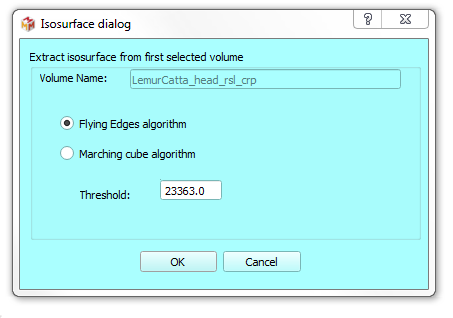
\includegraphics[scale=0.5]{images/14/isosurface/isosurface_dialog.png}
\caption{Isosurface dialog. A threshold value must be provided. You can either reconstruct the isosurface using the flying edges algorithem or the marching cubes algorithm.}	
\label{isosurface_dialog}
 \end{figure}

An example of isosurface extraction out of 3D volume data is provided Fig. \ref{isosurface_example} p.\pageref{isosurface_example}.
\begin{figure}
  \centering
  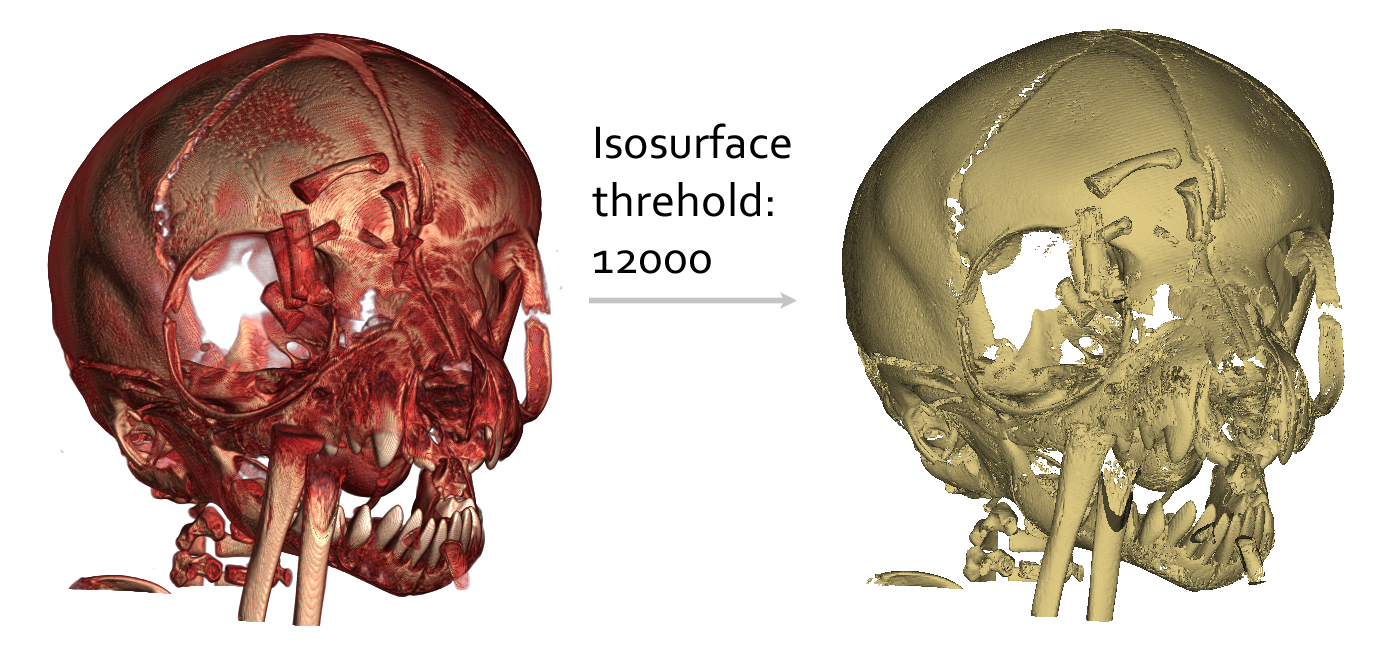
\includegraphics[scale=0.5]{images/14/isosurface/isosurface_lemur_catta_t12000.png}
\caption{Isosurface extraction example. \textbf{Left:} volume rendering representation of the cranium of a newborn \textsl{Lemur catta}. \textbf{Right:} 3D isosurface (threshold: 12000).}	
\label{isosurface_example}
 \end{figure}




\section{Flip or swap first selected volume}
This option opens the "Flip or Swap exes" dialog (see Fig. \ref{flip_swap_dialog} p.\pageref{flip_swap_dialog}). Flipping any of the axes will result in the production of a mirror image of the volume (see for instance Fig. \ref{flip_y_example} p.\pageref{flip_y_example}).
 
\begin{figure}
  \centering
  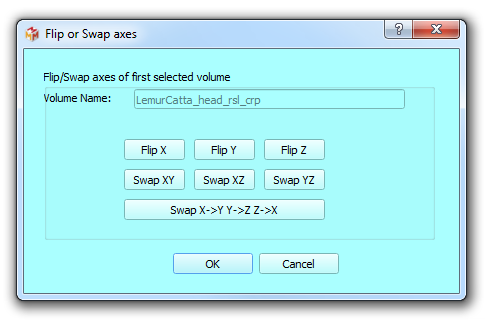
\includegraphics[scale=0.5]{images/14/flip_swap/flip_swap_dialog.png}
\caption{Flip or Swap axes dialog. You may decide either to flip an axis, or to swap 2 or 3 axes.}	
\label{flip_swap_dialog}
 \end{figure}


\begin{figure}
  \centering
  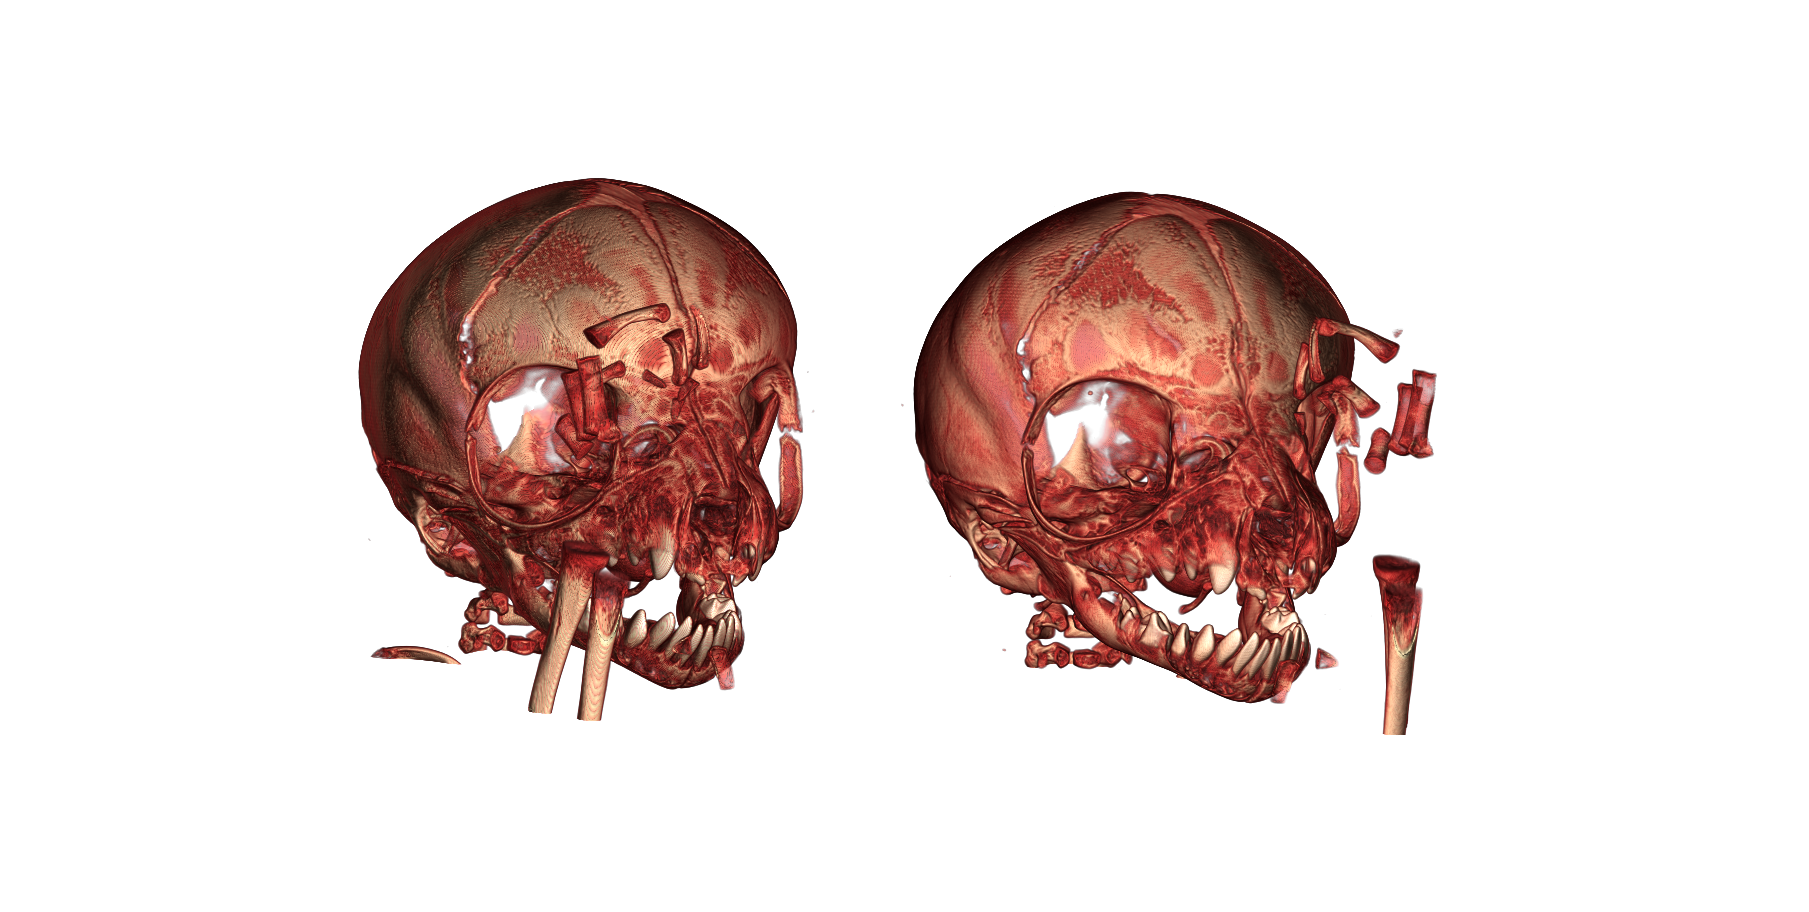
\includegraphics[scale=0.5]{images/14/flip_swap/flip_y_example.png}
\caption{ Example of axis Y flipping. Left: volume rendering representation of the cranium of a newborn Lemur catta. Right: the same volume rendering representation after axis Y was flipped.}	
\label{flip_y_example}
 \end{figure}



\section{Change voxel size of first selected volume (keep dimensions, no resampling}

\section{Resample first selected volume (dimensions will be changed, and voxel size as well)}

\section{Reslice first selected volume}

\section{Median filter of first selected volume}

\section{Gaussian filter of first selected volume}

\section{Invert first selected volume}

